%% 3 vertical dots
\vspace{1cm}

\begin{center}
{\hspace{1mm}\Large\vdots\hspace{1cm}}
\end{center}

\vspace{1cm}

%% Using units
\unit{10-300}{\mrad}

%% Sideways figure
\begin{sidewaysfigure}
  \begin{center}
  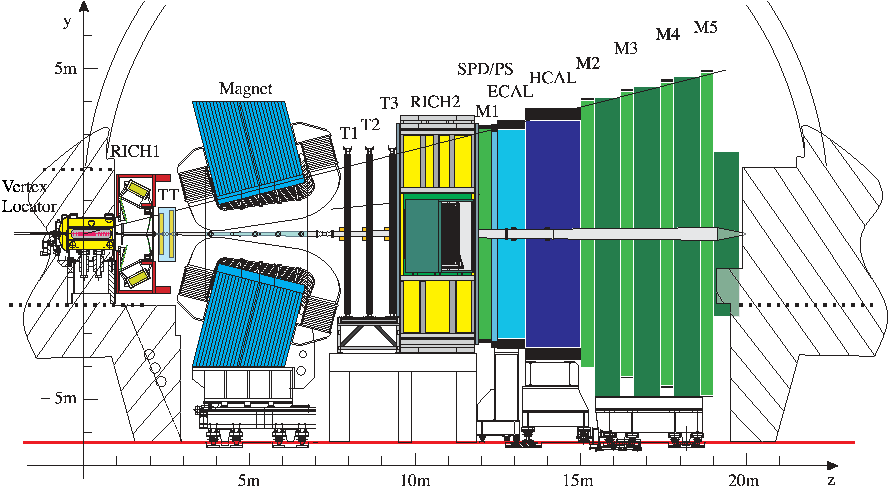
\includegraphics[width=0.8\textheight]{lhcb-detector-cross-section}
  \caption[Cross-section view of \LHCb, cut in the non-bending $y$--$z$ plane]%
    {Cross-section view of \LHCb, cut in the non-bending $y$--$z$ plane.}
  \label{fig:LHCbCrossSection}
  \end{center}
\end{sidewaysfigure}

%% Figure
\begin{figure}
  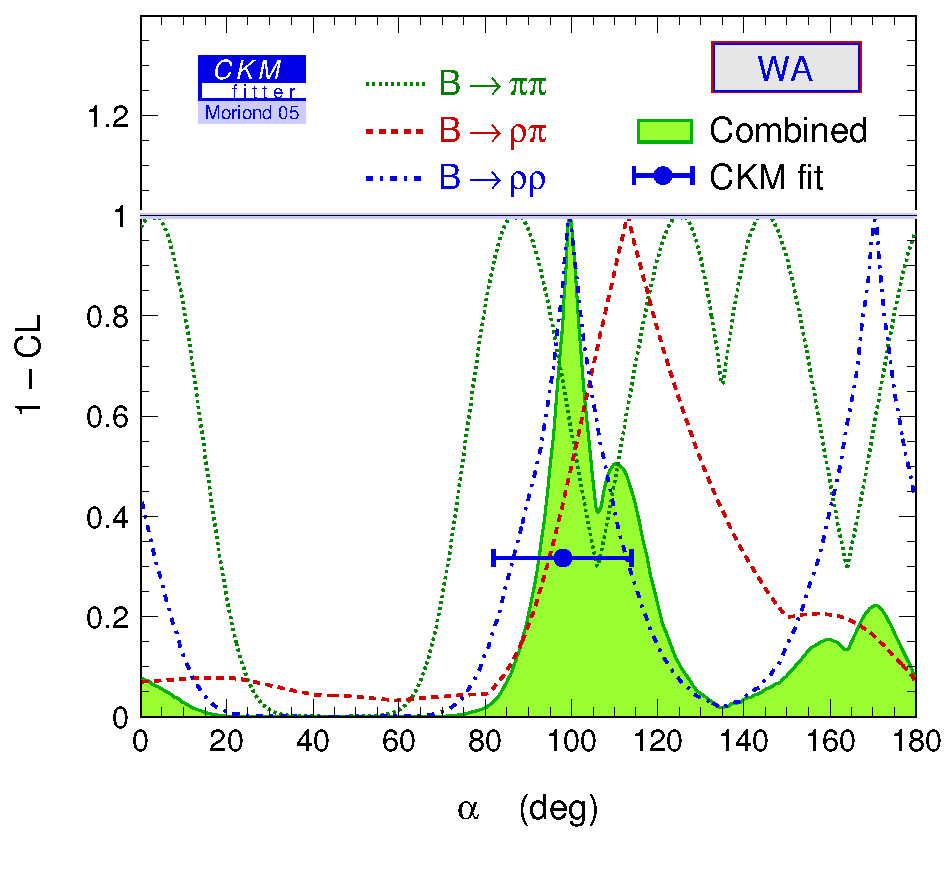
\includegraphics[width=\largefigwidth]{ckmfitter-alpha-combined}
  \caption[CKM Fitter constraints on \alphaCKM.]%
  {CKM Fitter constraints on \alphaCKM from combined \BToPiPi,
    \BToRhoPi and \BToRhoRho decay analyses.}
  \label{fig:CKMFitter}
\end{figure}

%% Approximation
\about{50\percent}

%% Equation
\begin{subequations}
  \label{eq:cosThetaCk}
  \begin{equation}
    \cos\,\thetaCerenkov  &= \frac{1}{n \beta} +
                             \frac{\hbar k}{2p}%
                             \parenths{ 1 - \frac{1}{n^2} } \\
                          &\,\sim \frac{1}{n \beta}%
    \label{eq:cosThetaCkApprox}
  \end{equation}
\end{subequations}


%
\begin{equation}
  \I \pdByd{}{t} \colvector{a \\ b}
  =
  \underbrace{%
  \twomatrix{ M_{11}-\frac{\I}{2}\Gamma_{11}
            & M_{12}-\frac{\I}{2}\Gamma_{12} }
            { M_{12}^\ast-\frac{\I}{2}\Gamma_{12}^\ast
            & M_{22}-\frac{\I}{2}\Gamma_{22} }
  }_{\boldmatrix{H}}
  \colvector{a \\ b}
  .
\end{equation}

%% Table
\begin{table}[bp]
  \begin{tabular}{lllll}
                & L0              & L1              & HLT             \\
    \midrule\\
    Input rate  & \unit{40}{\MHz} & \unit{1}{\MHz}  & \unit{40}{\kHz} \\
    Output rate & \unit{1}{\MHz}  & \unit{40}{\kHz} & \unit{2}{\kHz}  \\
    Location    & On detector     & Counting room   & Counting room   \\
  \end{tabular}
  \caption{Characteristics of the trigger levels and offline analysis.}
  \label{tab:TriggerDetails}
\end{table}